 \begin{itemize}
	\item {\textbf{Kratak opis:} Roba se utovara u kamion, kada je sve spremno vozach se upuc1uje ka destinaciji i oznachava da je proces dostavljanja porud2bine zapochet. Korisnik ima informaciju o tome da je vozach krenuo i gde se nalazi. Vozach nakon pristizanja na destinaciju oznachava zavrshetak procesa
		dostavljanja. }
	\item{\textbf{Ucesnici:} Vozach, Administrator}
	\item{\textbf{Preduslovi:} Narudzbina je primljena i obrad1ena  i roba  utovarena u kamion}
	\item{\textbf{Postuslovi:} Kamion je  stigao na destinaciju i spreman je za istovar}
	\item{\textbf{Osnovni tok:}  \begin{enumerate}
				\item {Vozach oznachava pochetak prevoza}
				\item {Vozach prevozi robu do zheljene destinacije}
				\item{Vozach pravi pauzu \begin{itemize} 
						\item [3.1]{Ukoliko vozach ne pravi pauzu tok se nastavlja }
						\item[3.2]{Ukoliko vozach pravi pauzu izvrshava se podtok P{1}}
				\end{itemize}
			}
				\item {Vozach oznachava kraj prevoza}
	\end{enumerate}}
\item{\textbf{Alternativni tok:} }

\item{\textbf{Podtokovi:}
		\begin{enumerate}
		\item {Vozach pravi pauzu : \begin{itemize}
					\item [P{1}]{Pauza je kratka, za gorivo ili lichne potrebe, nakon chega se izvrshava osnovni tok 2} 
					\item[P{2}]{U sluchaju nezgode ili kvara vozach obavestava administratora, koji izvrshava potrebne akcije i obaveshtava klijenta}
					\end{itemize}}
	\end{enumerate}}
\item{\textbf{Specijalni zahtevi:} Vozach poseduje ured1aj kojim mozhe da komunicira sa administratorom}
\item{\textbf{Dodatne informacije:}Vozach se identifikuje jedinstvenim brojem vozacha koji je vezan za broj kamiona}
\end{itemize}
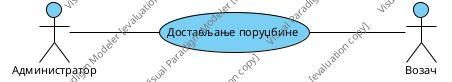
\includegraphics{Slike/SUdostavljanjePorudzbineUseCase}






